\documentclass{swp1}
\usepackage[utf8]{inputenc}
\usepackage{amssymb}
\usepackage{url}


% Tabellen
\usepackage{tabularx}
\usepackage{supertabular}
\usepackage{booktabs}







\begin{document}

% \maketitle{Nummer}{Abgabedatum}{Tutor-Name}{Gruppennummer}
%           {Teilnehmer 1}{Teilnehmer 2}{Teilnehmer 3}
\maketitle{2}{01.06.2014}{Michaela Bunke}{ChronoX}
          {Tim Ellhoff}{}{}
          
\section*{Aufgabe 1)}

Prototypen sind eine Art Vor- oder Zwischenprodukt in der Entwicklung, das dem finalen Produkt einerseits schon sehr oder auch nur zum Teil ähnlich sein soll. Sie können aber auch verwendet werden, um das noch nicht vorhandene Endprodukt in seinen Grundzügen oder Teilausschnitten vorab und günstig zu repräsentieren.\\
Ziel des Prototypings ist es zum einen, anhand eines praxisnahen Beispiels die Anforderungen zu ermitteln und zu überprüfen und zum anderen, die technischen Möglichkeiten unter die Lupe zu nehmen und aufzuzeigen. 

Unterscheidbar sind die Arten der Prototyp-Erstellung vor allem in der jeweiligen Lebensdauer. Im Allgemeinen kann man festlegen:\\

- \textbf{Wegwerf-Prototypen} (Grobe oder gar ohne Implementierung, Bloße Visualisierungen von Basisfunktionen) \\

- \textbf{Wiederverwertbare Prototypen} (Implementierung wird übernommen oder ausgearbeitet und angepasst)\\

- \textbf{Unvollständige Prototypen}  (Vorstellung von Teilfunktionen oder einzelnen Aspekten)\\

- \textbf{Vollständige Prototypen}  (Verfügbarkeit der wesentlichsten Funktionen)\\

Genauer werden die Arten im Folgenden festgelegt und beschrieben:\\

\begin{itemize}
\item \textbf{Explorativer Prototyp}
 
Das \textbf{Ziel} beim explorativen Prototyp ist in erster Linie die Lückenlosigkeit der Spezifikation zu überprüfen, durch Vorstellung der Anforderungen mit einer ersten grafischen Benutzerschnittstelle gegenüber dem Kunden/ Anwender, wobei das Augenmerk auf die bloße Funktionalität gelegt wird. Somit gehört der explorative Prototyp zu den Wegwerf-Prototypen\\
Durch diese Art der Vorgehensweise resultieren folgende Vor- und Nachteile.\\

\textbf{Vorteile:}
\begin{itemize}
\item Die Dauer der Entwicklung dieses Prototyps ist im Gegensatz zu den folgenden Arten der Prototyp-Bildung meist kurz und dient dazu, dem Kunden/ Anwender die Materie durch erste Visualisierungen greifbar zu machen und um Probleme zu veranschaulichen sowie diese im Anschluss direkt zu diskutieren.
\end{itemize}

\begin{itemize}
\item Die Qualität des Prototyps ist unerheblich und dadurch muss der Entwickler nicht zwingend genaue Detailkenntnisse besitzen und kann dennoch einen Prototypen erstellen und  vorstellen.
\end{itemize} 

\begin{itemize}
\item Die Kommunikation zwischen Entwickler und Auftraggeber wird erhöht und der Kunde/ Anwender kann direkt Einfluss auf das Projekt nehmen durch Validierung, Revidierung und Äußerung von Ideen und Wünschen. 
\end{itemize}

\begin{itemize}
\item Der Entwickler kann durch das Annehmen neuer Ideen und Wünsche, was einen Mehraufwand bedeuten kann, erneut Arbeitsbedingungen verhandeln. 
\end{itemize}

\textbf{Nachteile:}
\begin{itemize}
\item Größter Nachteil ist die, durch den kurzen Zyklus der Entwicklung und der Art des Prototyps entstandenen Oberflächlichkeit. Dies bedeutet, dass im Vorfeld geklärt werden muss, ob diese Art des Prototyps angebracht ist oder nicht, da relevante Anforderungen innere Prozesse sein können die nicht sichtbar gemacht werden können. 
\end{itemize}

\begin{itemize}
\item Der Funktionsumfang kann unnötig vergrößert werden durch neue Wünsche, die nicht unbedingt sinnvoll sein müssen.
\end{itemize}

\item \textbf{Evolutionärer Prototyp}

Das \textbf{Ziel} beim evolutionären Prototyp ist der genauere Ausbau eines lauffähigen System in mehreren Schritten oder Teilen, angefangen bei einem einfachen Prototyp. Der Prototyp kann dem Zielsystem angepasst oder zum Zielsystem ausgebaut werden und erhält dadurch eine lange Lebensdauer und gehört somit zu den wiederverwertbaren Prototypen.


\textbf{Vorteile:}

\begin{itemize}
\item Schnelle Bereitstellung eines lauffähigen Systems möglich, da vom Anfangs- oder Startprototypen keine vollständige Funktionalität erwartet wird und diese in den nächsten Versionen vervollständigt werden können.
\end{itemize}

\begin{itemize}
\item Fehlende oder mangelnde Anforderungen können in mehreren Versionen Schritt für Schritt hinzugefügt oder verbessert werden.
\end{itemize}


\begin{itemize}
\item In den einzelnen, aufeinander aufbauenden Schritten können Zwischenergebnisse ausgearbeitet werden, die zugleich validiert werden können. Dadurch verringert sich das Risiko einer Fehlentwicklung drastisch, zumal der Auftraggeber in den Zwischenergebnissen mit einbezogen wird.
\end{itemize}

\textbf{Nachteile:}
\begin{itemize}
\item Nach jeder Validierung findet eine Planung statt, bei der fehlende Teile und die nächsten Schritte besprochen werden müssen. Demnach wird eine Versionsverwaltung erfordert, die erschwerend für das Projekt sein kann.
\end{itemize}

\begin{itemize}
\item Die Unübersichtlichkeit ist bei großen Projekten gegeben, da die Schnittstellen für die Versionen oder Teilprojekte sich laufend ändern können.
\end{itemize}

\item \textbf{Experimenteller Prototyp}

Das \textbf{Ziel} beim experimentellen Prototyp ist im Allgemeinen eine Überprüfung von verschieden Aspekten in einem Projekt und die Forschung. Hier werden Möglichkeiten für die Umsetzung gesucht und Lösungsideen überprüft. Teilentwürfe und Architekturmodelle werden ebenfalls überprüft und Machbarkeitsstudien können ebenfalls durchgeführt werden. Dadurch haben diese Prototypen eine geringe Lebensdauer und sind generell Wegwerf-Prototypen.\\

\textbf{Vorteile:}
\begin{itemize}
\item Durch den experimentellen Aspekt dieses Prototyps entsteht einfaches Learning-by-Doing („Lernen durch Handeln“).
\end{itemize}

\begin{itemize}
\item Kann wirtschaftlich sein, wenn durch schnelle und neu gewonnene Erkenntnisse Kosten in der Entwicklung eingespart werden können.
\end{itemize}

\begin{itemize}
\item Ergebnisse können als Grundlage für eine Risikoeinschätzung dienen.
\end{itemize}

\begin{itemize}
\item Durch den experimentellen Aspekt müssen Implementierungen nicht sauber sein, sondern eher schnell.
\end{itemize}

\begin{itemize}
\item Simulationen oder Vergleiche von fehlerhaften oder unwichtigen Algorithmen/ Teilen können durchgeführt werden.
\end{itemize}

\begin{itemize}
\item Ergebnisse können als Grundlage für eine Risikoeinschätzung dienen.
\end{itemize}


\textbf{Nachteile:}
\begin{itemize}
\item Durch schlecht durchdachte Ansätze können schnell Ressourcen verschwendet werden und experimentelle Prototypen können meist in keiner Weise weiterverarbeitet oder ausgebaut werden können.
\end{itemize}


\end{itemize}

\subsection*{a) und b) (in einem Text)}
Zunächst lassen sich Prototypen in zwei Kategorien einteilen. Zum einen gibt es sie in Bezug auf die Lebensdauer und zum anderen in Bezug auf den Zweck. Unterschieden werden kann bei der Funktionalität, da es die horizontale Richtung, in der bestimmte Ebenen wie Anwendungslogik oder Benutzerschnittstelle möglichst vollständig abgedeckt werden, und die vertikale Richtung, die darauf abzielt, Teilbereiche aller Ebenen des Systems zu erfassen, zum Beispiel bei so genannten kritischen Anforderungen. \\
Außerdem gibt es noch bestimmte Typen von Prototypen; den Papierprototypen, der selbst keine Interaktion bietet, analytisch ausgelegt ist und meist durch Screenshots oder Bildschirmmasken visualisiert wird und simple Ein- und Ausgabemöglichkeiten der Software präsentiert; dann den animierten Prototypen, der ein Systemverhalten zeigt, das als eine Art Demo selbstständig läuft; und den interaktivsten, nämlich den ausführbaren Prototypen, der natürlich auch am teuersten und aufwändigsten ist, aber auch die meisten Funktionen wie z.B. echtes GUI-Design bietet.\\

\subsubsection*{Wegwerf-Prototyp}
Bezüglich der Lebensdauer ist der Wegwerf-Prototyp zu nennen, der, wie der Name schon verrät, nicht weiterentwickelt wird, sondern nur bezogen auf einen gewissen Ausschnitt eingesetzt wird, um z.B. ein bestimmtes Feature zu untersuchen oder Funktionalitäten zu repräsentieren. Dabei wird meist darauf geachtet, dass diese Art von Prototyp kostengünstig zustande kommt, was natürlich schon vermuten lässt, dass dieser auch nur für kurze Zeit verwendet und für spätere Versionen bzw. Stufen im Projekt unbrauchbar sein wird. Er wird regelrecht verworfen.\\
Man könnte so einen Prototypen beispielsweise einsetzen, um im Kundengespräch den Dialog zu fördern oder das ggf. noch nicht vorhandene Verständnis vom zu erstellenden Produkt, also der Software, dem Kunden näher zu bringen bzw. dieses zu visualisieren. Dabei kann es auch nur auf ganz spezielle Dinge oder Funktionalitäten ankommen und andere, zwar im Gesamtzusammenhang auch wichtige, aber für den Moment zu vernachlässigende Dinge können durchaus bei dieser Art des Prototypings vollkommen ausgeblendet werden. Somit kann auch eine gewisse Ungenauigkeit bzw. Unvollständigkeit an den Tag gelegt werden. Es geht vielmehr darum, gezielt bestimmte, vielleicht noch unklare Anforderungen oder Wünsche dem Kunden mittels des Prototypen zu entlocken.\\
Ein großer Vorteil des dabei ist, dass schon sehr früh im Projekt nützliche Lösungsansätze herausgearbeitet werden, auf die man auch später wieder zurückgreifen kann. Wegwerf-Prototypen sind häufig auch ohne großen Aufwand zu realisieren. Auch helfen sie, den Kunden bzw. Benutzer schon sehr früh am Produkt bzw. an dessen Entwicklungsprozess zu beteiligen und ggf. ein nützliches und verwertbares Feedback zu erhalten, was die Risiken von frühzeitigen Fehlentwicklungen deutlich abschwächen kann. Das dient auch der Kommunikation mit dem Kunden.\\
Nachteile sind, dass man vorher schon weiß, dass er verworfen wird, woraus sich ggf. gewisse Ungenauigkeiten bzw. mangelnde Sorgfalt schon beim Erstellen des Protypen ergeben können. Außerdem werden nur bestimmte Bereiche betrachtet, während andere, vielleicht auch wichtige Bereiche, ignoriert und ausgeblendet werden. Der Blick auf das "große Ganze" fehlt hier.

\subsubsection*{Evolutionärer Prototyp}

Ein zweites, z.T. gegensätzliches Beispiel bezüglich der Lebensdauer ist der evolutionäre Prototyp, der hingegen nicht verworfen, sondern Schritt für Schritt weiterentwickelt und allmählich zum Endprodukt ausgebaut wird. Er muss daher gerade in Bezug auf Vollständigkeit ganz anderen Qualitätsanforderungen genügen als der Wegwerf-Prototyp, was nicht heißt, dass er schon zu Beginn an komplettiert sein muss. Er müssen vielmehr alle Anforderungen des zu erstellenden Systems grob miteinbezogen worden sein. Der Vorteil hierbei ist, dass jedes Inkrement gewissermaßen eine neue Stufe darstellt, auf deren Basis der Kunde bzw. Benutzer diesen testen und sein persönliches Feedback abgeben kann, wovon auch die jeweiligen Weiterentwicklung entscheidend abhängen. Typische Inkremente können sich in grundlegende, erweiterbare, zusätzliche und ergänzende Funktionalitäten hierarchisieren lassen. \\
Diese Art von Prototyp lässt sich zum Beispiel sehr gut in größeren Projekten wie SWP2 anwenden, indem auf Basis eines evolutionären Prototyps, der ggf. für das Stundenplansystem zur Verfügung gestellt wird, die Software mithilfe von grundsätzlichen und frühen Kommunikationsmöglichkeiten mit dem Kunden und dessen aktive Mitgestaltung  weiterentwickelt werden kann, was auch die Akzeptanz und das Verständnis des Kunden erhöhen kann, da er ständig in den Projektprozess involviert wird und das Risikos des Fehlentwicklung senkt.\\
Natürlich kann es auch aufgrund des mangelnden technischen Verständnisses des Kunden passieren, dass der Kunde eine verfrühte Einschätzung bezüglich des Entwicklungsfortschritts des Produktes entwickelt und ggf. die noch aufkommende Arbeit und Dauer des Projekts unterschätzen.

\subsubsection*{Technischer Prototyp}

Wie oben schon erwähnt, gibt es neben der Lebensdauer eine weiteren Bezug, die Prototypen nehmen können: den Zweck. Als Beispiel sei hier der technische Prototyp genannt, der darauf abzielt, die technische Realisierbarkeit von den Ansätzen zu der vollständigen Problemlösung zu untersuchen und darzustellen. Hier geht es nicht darum, Systeme vollständig zu implementieren, sondern gezielte Teilbereiche herauszugreifen, an deren Prototypen man die technische Machbarkeit des jeweiligen Features abschätzen kann, wobei es  hierbei je nach genauer Zielsetzung sowohl Wegwerf- als auch evolutionäre Modelle geben kann. \\
Man könnte diesen Prototypen einsetzen, um eine bestimmte Funktionalität, die man im System implementieren möchte, im Stundenplan-Projekt auf seine Machbarkeit zu untersuchen. Dabei kann es ja sein, dass man spezielle Features ggf. optionaler Art unbedingt ins System integrieren möchte, aber nicht genau einschätzen kann, ob dies auch technisch realisierbar ist. Hier kann so ein Prototyp dazu dienen, dies herauszufinden.\\
Die Vorteile liegen auf der Hand: Lange und ggf. vergebliche Implementierungs- und Entwicklungsprozesse bleiben aus, wenn das technische Prototyping bezüglich der Realisierbarkeit negativ ausfällt, was den Fokus der Entwickler auf andere Dinge richten lässt. Nachteilig ist, dass auch dieser Prototyp eher speziell ist und nicht für das ganze System genutzt werden kann, das für den Gesamtüberblick nicht ideal ist. 
 
\section*{Aufgabe 2)}
GUI für das Stundenplansystem
\clearpage


\begin{figure}
\centering{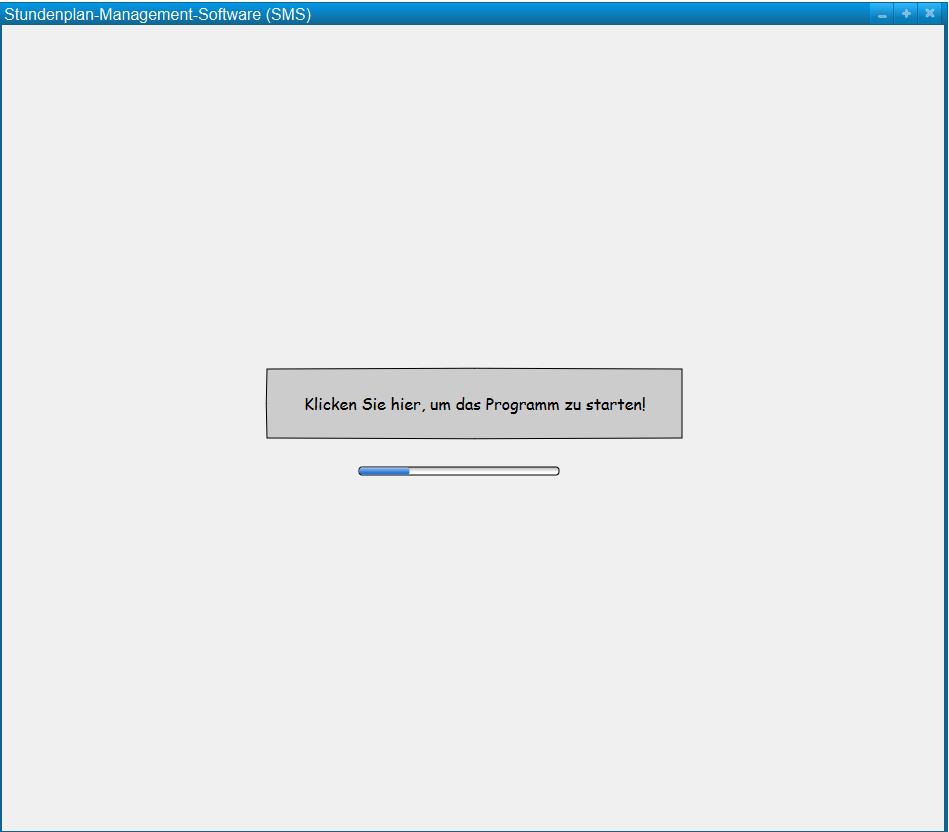
\includegraphics[width=\textwidth] {GUI/1.png}}
\caption{Startseite des Stundenplansystems }
\label{ab1}
\end{figure}

\begin{figure}
\centering{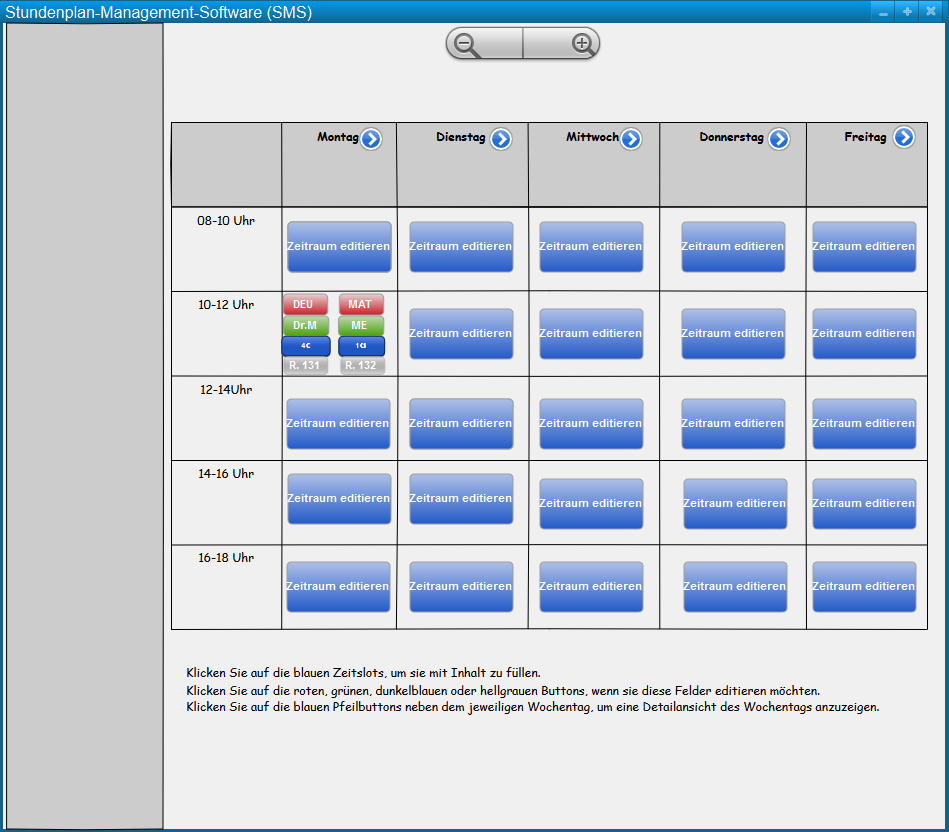
\includegraphics[width=\textwidth] {GUI/2.png}}
\caption{Wochenübersicht mit vielen freien (blauen) Zeitslots. Nur Montag von 10-12 Uhr laufen zwei parallele Veranstaltungen. Durch einen Klick auf einen der bunten Buttons öffnet sich eine Sidebar zur Bearbeitung.}
\label{ab2}
\end{figure}

\begin{figure}
\centering{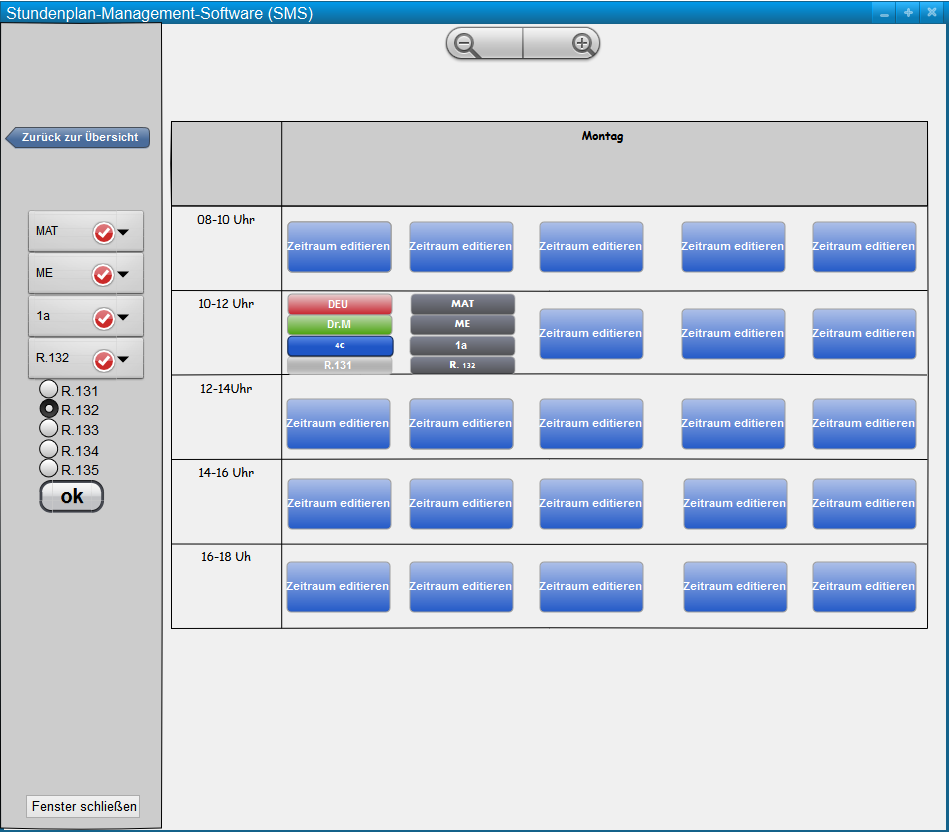
\includegraphics[width=\textwidth] {GUI/2a.png}}
\caption{Detailübersicht für den Montag: die anthrazitfarbenen Buttons sind zur Bearbeitung in der linken Sidebar geöffnet und können editiert werden. }
\label{ab3}
\end{figure}

\begin{figure}
\centering{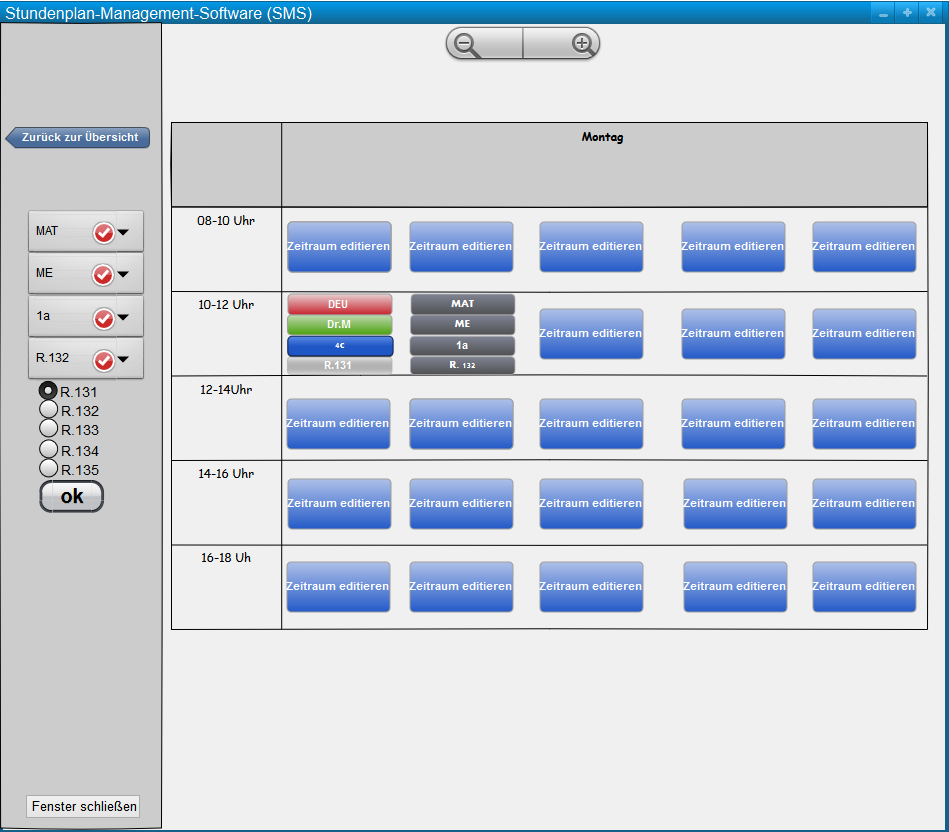
\includegraphics[width=\textwidth] {GUI/2b.png}}
\caption{Jetzt wurde links der Raum 131 angewählt. }
\label{ab4}
\end{figure}

\begin{figure}
\centering{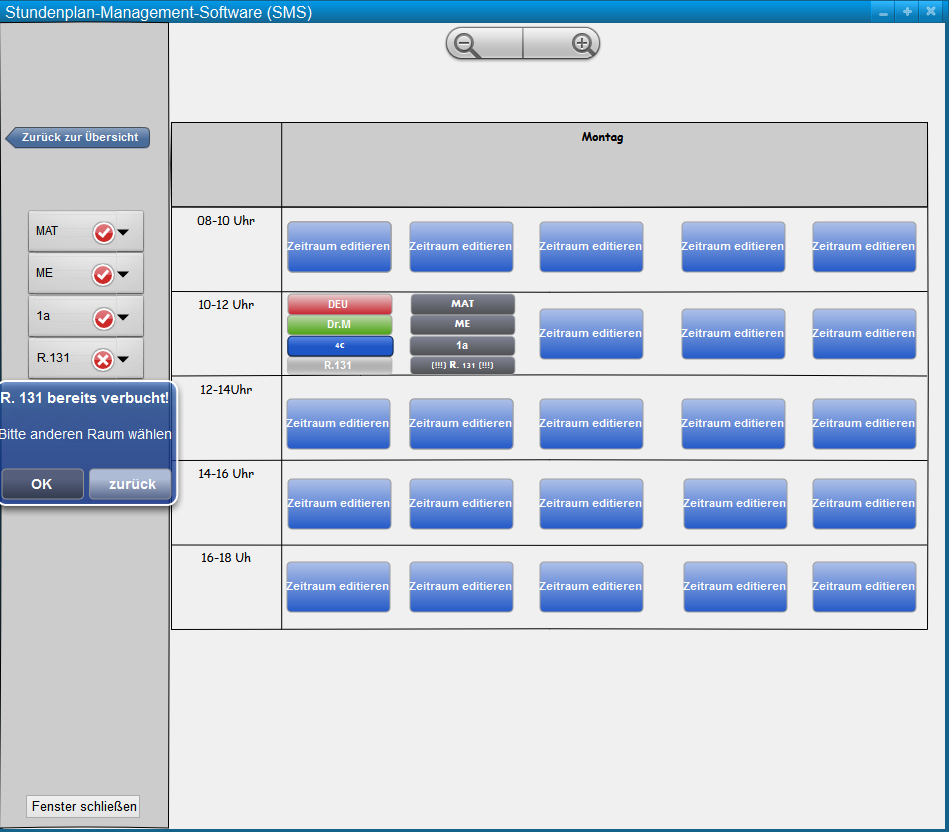
\includegraphics[width=\textwidth] {GUI/3.png}}
\caption{Jetzt erscheint eine Fehlermeldung, dass der gewünschte Raum bereits belegt ist (zeitgleich mit dem Deutschkurs). Der Nutzer hat die Möglichkeit, im nächsten Schritt den Raum zu ändern oder zurückzugehen.}
\label{ab5}
\end{figure}

\begin{figure}
\centering{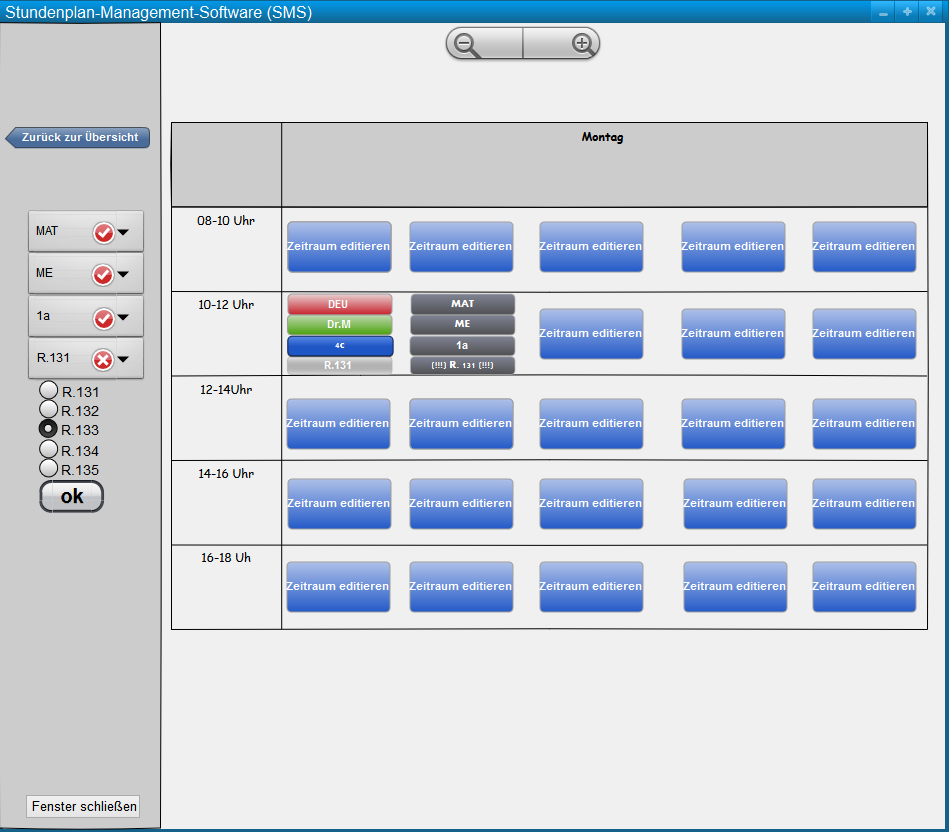
\includegraphics[width=\textwidth] {GUI/3a.png}}
\caption{Der Nutzer hat sich entschlossen, Raum 133 auszuwählen und klickt OK. }
\label{ab6}
\end{figure}

\begin{figure}
\centering{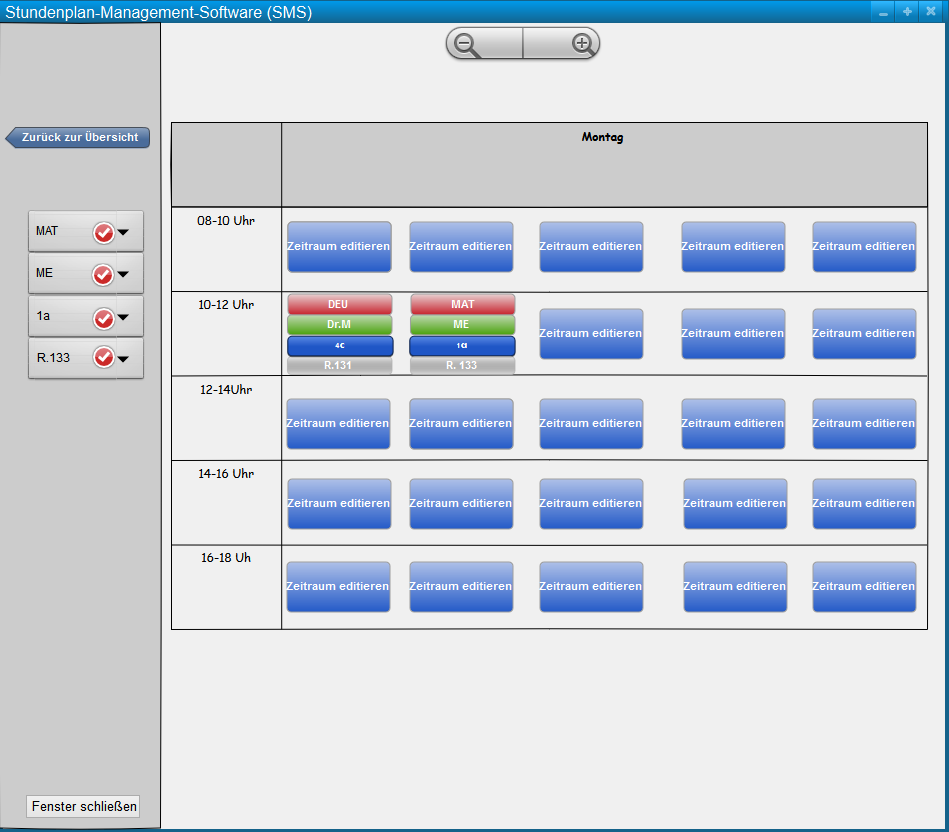
\includegraphics[width=\textwidth] {GUI/3b.png}}
\caption{Das System akzeptiert die Auswahl. Jetzt stehen links in der Sidebar überall Häkchen und kein Kreuz mehr und die Farben wurden auch wieder von anthrazit auf die bunten Ausgangsfarben im Stundenplan geändert. }
\label{ab7}
\end{figure}

\begin{figure}
\centering{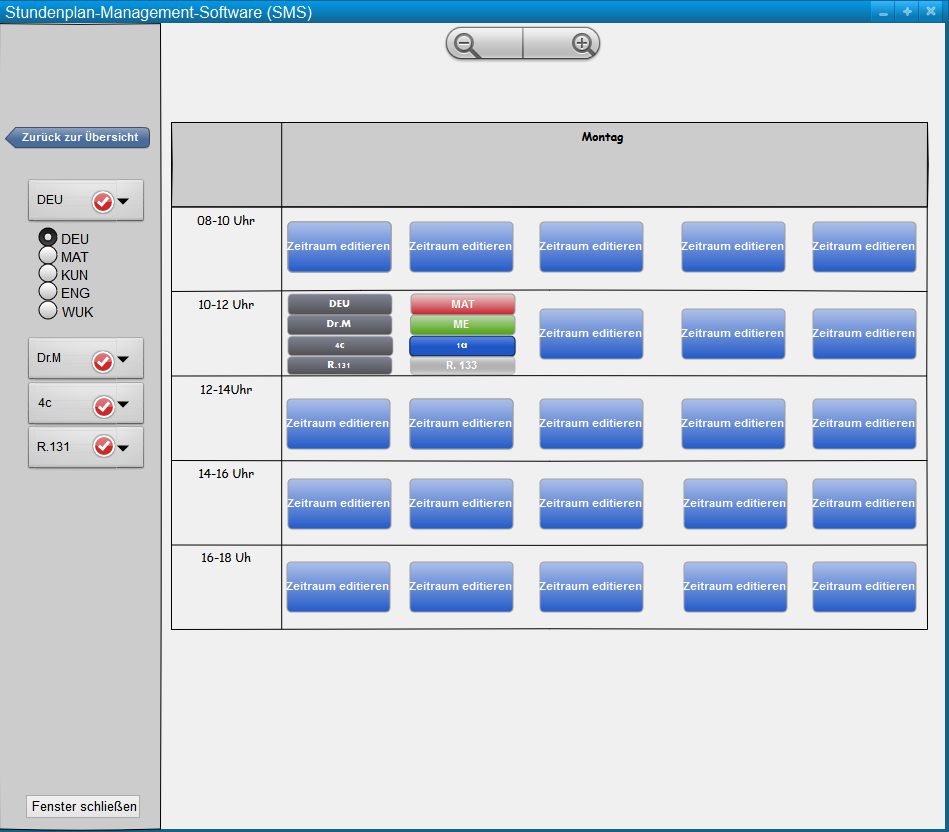
\includegraphics[width=\textwidth] {GUI/4.png}}
\caption{Der Nutzer entscheidet sich jetzt, den Deutschkurs zu editieren.Ein Unterauswahlmenü mit verschiedenen Fächern erscheint. }
\label{ab8}
\end{figure}

\begin{figure}
\centering{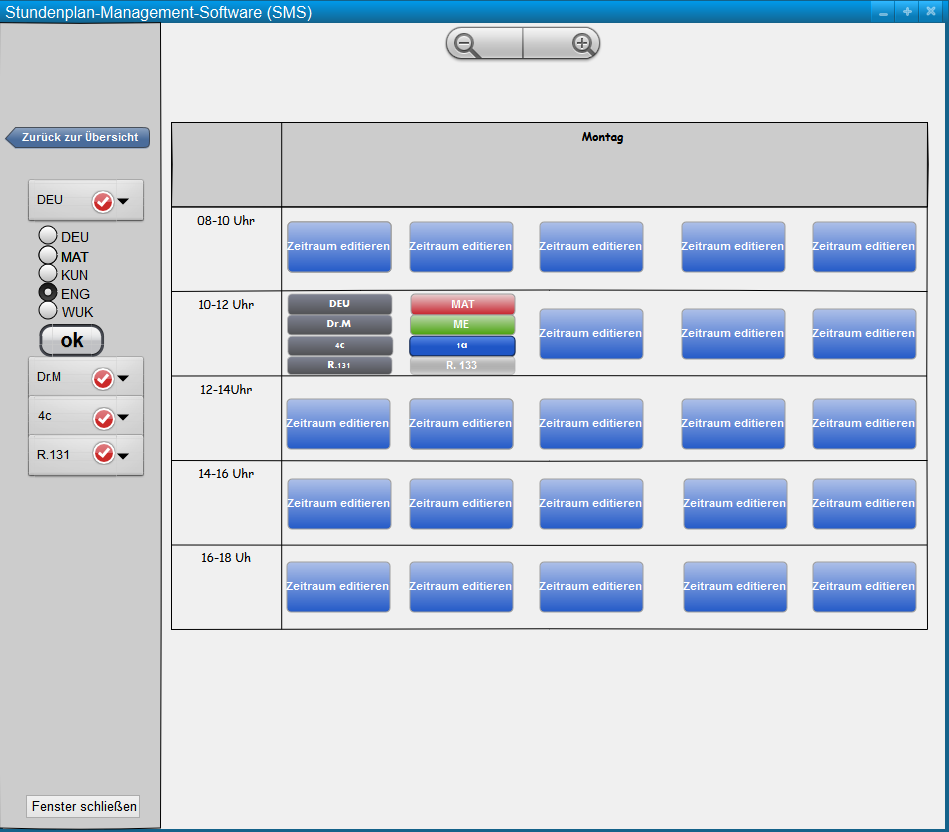
\includegraphics[width=\textwidth] {GUI/4a.png}}
\caption{Er wählt als Fach Englisch aus und klickt OK. }
\label{ab9}
\end{figure}

\begin{figure}
\centering{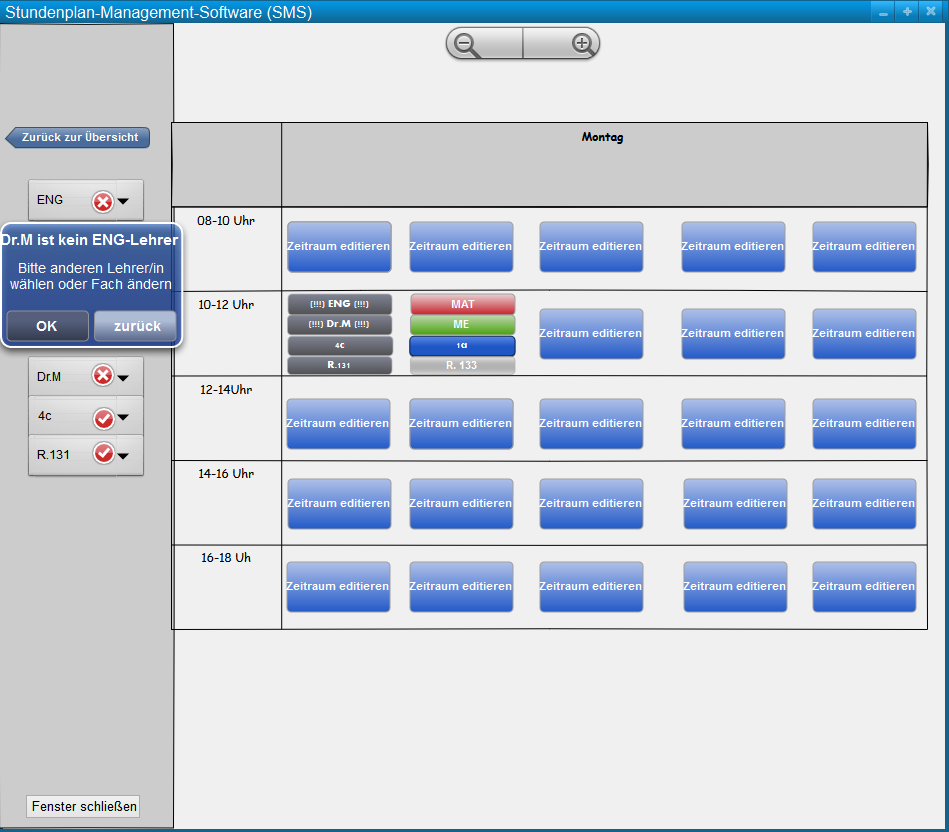
\includegraphics[width=\textwidth] {GUI/4b.png}}
\caption{Nun stört sich das System daran, dass Lehrer Dr.M kein Englischlehrer ist. Der Nutzer kann entweder den Lehrer oder das Fach ändern (oder zurückgehen). }
\label{ab10}
\end{figure}

\begin{figure}
\centering{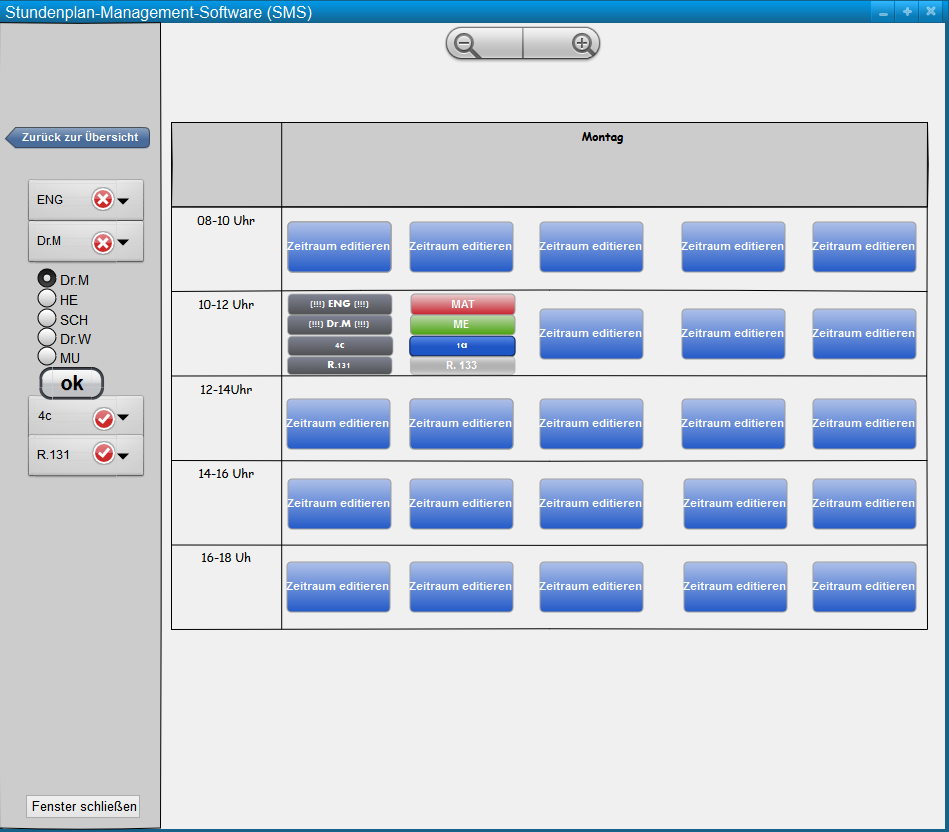
\includegraphics[width=\textwidth] {GUI/4c.png}}
\caption{Wenn er die Eingabe so belässt, wird das System wieder einen Hinweis geben. Das erkennt man an den roten Kreuzen links in der Sidebar und auch an den Ausrufezeichen (!!!) im Stundenplan macht uns das System darauf aufmerksam, dass die Belegung nicht korrekt ist. Also muss er die Auswahl ändern.}
\label{ab11}
\end{figure}

\begin{figure}
\centering{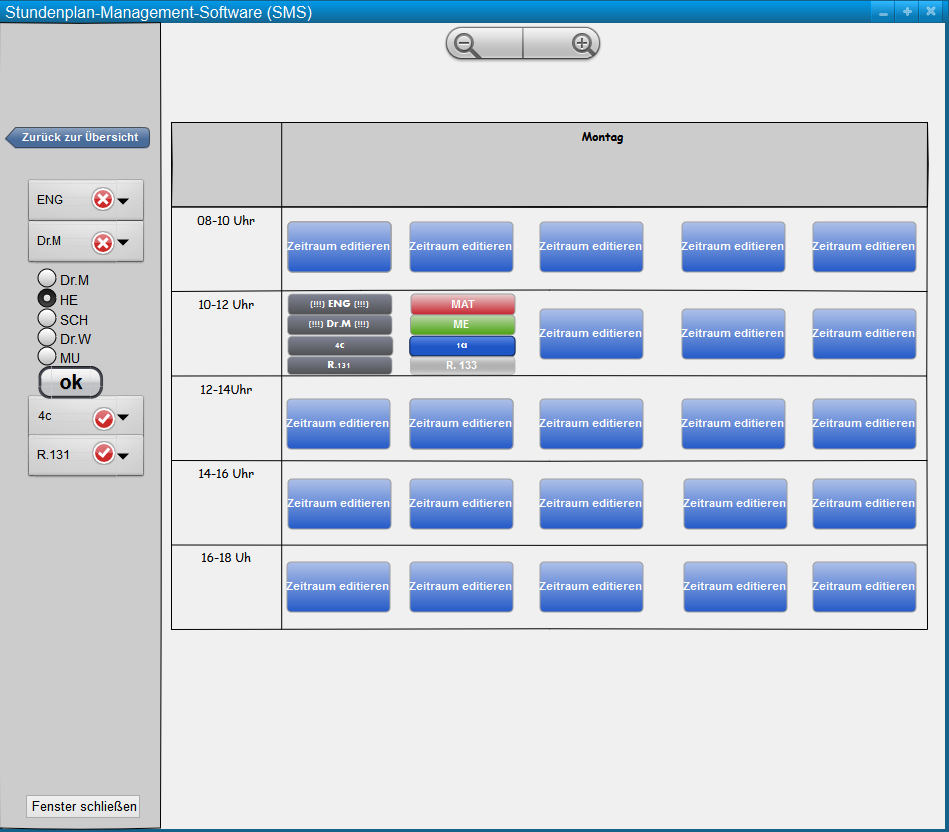
\includegraphics[width=\textwidth] {GUI/4d.png}}
\caption{Der Nutzer ändert den Lehrer auf Frau/Herrn He. und klickt OK (in der Auswahlliste waren alle verfügbaren Englischlehrer). }
\label{ab12}
\end{figure}

\begin{figure}
\centering{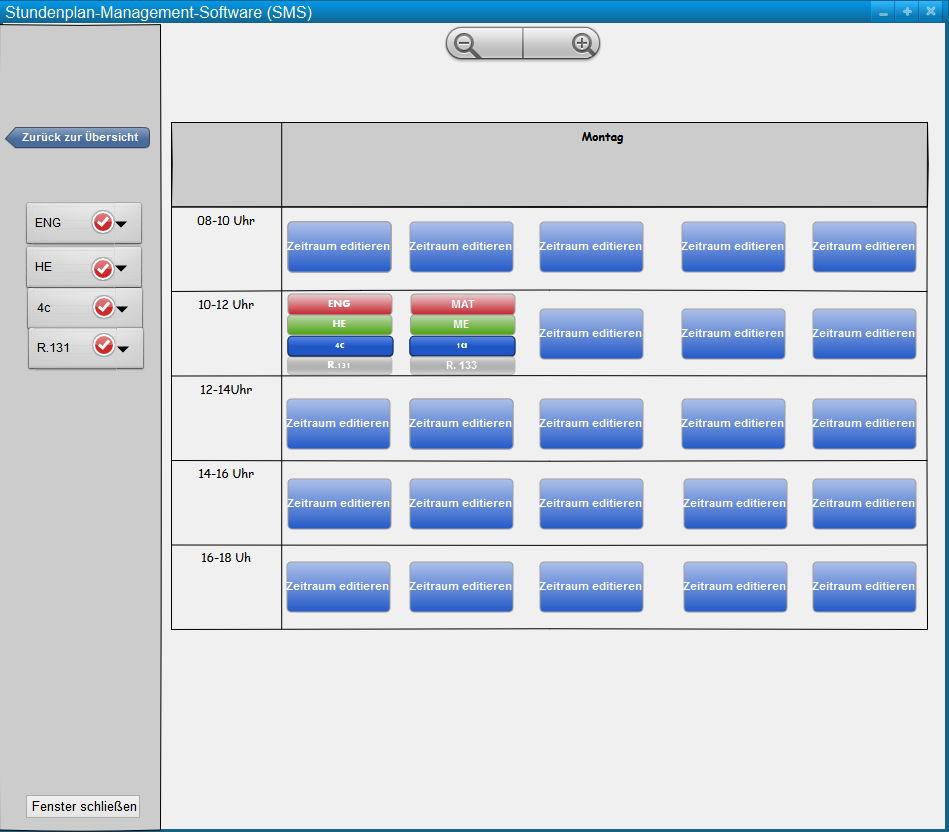
\includegraphics[width=\textwidth] {GUI/4e.png}}
\caption{Die Eingabe wird akzeptiert und das System gibt keine Fehlermeldungen mehr aus. }
\label{ab13}
\end{figure}



\section*{Aufgabe 3)}

	
	\begin{tabular}
		{|p{5cm}|p{10cm}|} \hline \textbf{1} & \textbf{Editieren einer Aktivität im Stundenplan} \\
		\hline \textbf{Akteure} & Ludwig Lehrer, Otto Oberstufenkoordinator, Detlef Direktor\\
		\hline \textbf{Ziel} & Der Akteur möchte eine Aktivität im Stundenplan editieren. \\
		\hline \textbf{Vorbedingungen} & keine \\
		\hline \textbf{Regulärer Ablauf} & 1. Der Akteur startet das Stundenplan-Management-Programm mittels des Buttons (siehe Abbildung \ref{ab1}). \\
		&2. Das Programm startet und zeigt die Hauptseite mit einer Übersicht (siehe Abbildung \ref{ab2}). \\
		&3. Der Akteur klickt auf einen der bunten Buttons im Zeitslot 10-12 Uhr am Montag. \\
		&4. Die Seite wird angezeigt. In dem jetzt zu sehenden Stundenplanauschnitt für Montag hat der Akteur durch Klicken auf bestimmte Zeiträume folgende Möglichkeiten der Editierung:
		\begin{itemize}
		\item \texttt{Zeitraum von 10-12 Uhr (Deutschkurs) editieren}
		\item \texttt{Zeitraum von 10-12 Uhr (Mathekurs) editieren}
		\item \texttt{einen blauen freien Zeitraum editieren bzw. mit Inhalt füllen}
\end{itemize}	
(siehe Abbildung \ref{ab3}).	   
 Er wählt den Deutschkurs aus und es erscheint ein weiteres Auswahlmenü, wo Fächer, Lehrer, Klasse und Räume editiert werden können (siehe Abbildung \ref{ab4}).\\
&5. Wenn man alles korrekt eingegeben hat (siehe Abbildung \ref{ab6}) und OK klickt, wird die Eingabe akzeptiert (siehe Abbildung \ref{ab7}).\\
		\hline \textbf{Nachbedingungen} & Der Akteur sieht nun im Stundenplan die Belegung des gewünschten Zeitraums mit der gewünschten Aktivität. \\
		\hline \textbf{Fehler-/Ausnahmefälle} & Server ist nicht erreichbar bzw. das Programm lässt sich nicht fehlerfrei ausführen. \\
		\hline 
	\end{tabular}






\section*{Aufgabe 4)}

\subsubsection*{Wartbarkeit}
Diese Aussage ist ungenügend, weil sie viel zu allgemein formuliert ist und sich gar nicht erkennen lässt, was Wartbarkeit in dem Fall bedeuten soll bzw. auf was sich dieser Begriff genau bezieht. Sie ist viel zu ungenau und wird unweigerlich zu Missverständnissen zwischen Kunden und Entwicklern führen, wenn sie nicht korrigiert und konkretisiert wird. \\
Je nach Softwaresystem und Systemausrichtung kann Wartbarkeit Unterschiedliches bedeuten und muss im Gesamtzusammenhang gesehen werden. Es macht einen Unterschied, ob man unter Wartung die Beseitigung von Fehlern versteht, Reengineering- oder Refactoringmaßnahmen betrachtet oder die Software an veränderte (technische) Rahmenbedingungen anpassen möchte. \\
Wenn man softwareergonomische Prinzipien anwendet, könnte man die Aussage allgemein folgendermaßen umformulieren:\\
„Das System sollte von Grund auf modular aufgebaut, gut strukturiert und dokumentiert sein.
Desweiteren werden spätere Veränderungen am Produkt erwartet, wenn es nicht sogar als
Grundlage für ein weiteres Projekt gedacht oder recycelt werden soll. Es müssen auch Eingriffe in
das laufende System beim Kunden möglich sein.“

\subsubsection*{Performanz}
Ähnlich ungenau ist die zweite Aussage formuliert. Perfomanz, also Leistung, kann sich auch auf alles Mögliche beziehen, je nach dem, auf was das Softwaresystem abzielt und welche Prioritäten es setzt. Bezieht sich die Performanz auf die Leistung der einzelnen Software-Komponenten wie Ausschnitte einer Anwendungssoftware oder Betriebssystemteile oder geht es eher darum, z.B. bestimmte Rechenoperationen in Java so schnell und effizient wie möglich durch den passenden Algorithmus zu implementieren? All das ist hier völlig offen gelassen worden. Zumindest hätte eine grobe Richtung angeben müssen, auf was sich Performanz beziehen soll.
Umformuliert könnte man schreiben: „Das System soll so aufgebaut sein, dass die einzelnen Softwarekomponenten möglichst effizient in Bezug auf Geschwindigkeit der Datenverarbeitung und der Kommunikation untereinander arbeiten und gut miteinander harmonieren, sodass die Leistung, also die Performanz des Systems, möglichst hoch ist."


\section*{Aufgabe 5)}
\subsection*{a)}
Um das Kano-Modell zu verstehen, muss man sich zunächst darüber im Klaren sein, dass der Mensch und somit jeder Kunde bzw. Benutzer unterschiedliche Bewusstseinsebenen hat, auf Basis derer er handelt. So liegt es meist nicht an der Unkenntnis des Kunden, dass er nicht genau einschätzen kann, was er genau will oder sehr unstetig ist, sondern schlichtweg am Wissen, dass sich in drei Kategorien einteilen lässt: dem bewussten, dem unbewussten und dem unterbewussten Wissen.\\
Bei ersterem handelt es sich um das Wissen, was man klar realisiert und sich um dessen Bedeutung somit vollständig im Klaren ist. Das macht in etwa zwanzig bis dreißig Prozent des Wissens aus. \\
Das unbewusste Wissen hingegen ist nicht ständig präsent, aber doch so nah an die Oberfläche zu tragen ist, dass man es jederzeit abrufen kann und es auch als wichtig empfindet. Das macht mehr als vierzig Prozent aus.\\
Beim unterbewussten Wissen weiß man selbst ohne Außenwirkung gar nicht, dass man bestimmte Wünsche hat, die gerne erfüllt bekommen würde.\\

Diese drei Bewusstseinsebenen spielen auch bei der Anforderungsanalyse eine maßgebliche Rolle. Das Kano-Modell stellt hierbei gewissermaßen den direkten Zusammenhang zwischen Erfüllungsgrad der Anforderungen und der Kundenbegeisterung dar. Dabei gilt die logische Schlussfolgerung, dass ein hoher Erfüllungsgrad auch zu einer großen Begeisterung führt, wobei es je nach Anforderung auch sein kann, dass ein hoher Erfüllungsgrad keine Begeisterungsstürme auslöst, sondern nur das nüchterne Eintreten der Selbstverständlichkeit verursacht.\\
Das Kano-Modell unterteilt deshalb die Anforderungen in verschiedenen Faktoren. Die Basisfaktoren sind gewissermaßen die Mindestanforderungen für das System, die vom Kunden als klar erfüllt vorausgesetzt werden und dessen Nichterfüllung zu großer Unzufriedenheit und somit zu einem Ausschlusskriterium führt. Der Begriff Mindestanforderungen suggeriert schon, dass hier keine "Mehrerfüllung" erreicht werden kann. Entweder die Anforderungen sind erfüllt oder nicht. \\
Die zweite Stufe bilden die Leistungsfaktoren, bei deren Erfüllung der Kunden einem auch nicht etwa vor Freude um den Hals fällt, sondern im Gegenteil die Erfüllung dieser als bewusst verlange Ausstattung versteht, deren Nichterfüllung auf Unzufriedenheit stößt.\\
Begeistern kann man den Kunden nur, wenn man ihm etwas anbietet, mit dem er nicht gerechnet. Die so genannten begeisternden Faktoren drücken dies aus. Bei Erfüllung dieser ist der Kunde unverhältnismäßig zufrieden, sodass man als Entwickler ab dieser Stelle nur noch ''gewinnen'' kann. Selbst die Nichterfüllung führt nicht zu einer Unzufriedenheit, weil der Kunde ohne den Anstoß dieser Anforderungen von außen selbst niemals verlangt hätte.

\subsection*{b)}
Das Kano-Modell lässt sich für ein Software-Projekt gut anwenden, da es typische Aussagen über die Erfüllungsgrade der Anforderungen macht und diese aufbauend hierarchisiert. \\
Das Ziel in SWP2 ist klar die Erfüllung der Basisfaktoren, ohne die der Kunde völlig unzufrieden, die Software unbrauchbar und wir alle das Modul folgerichtig nicht bestanden hätten. Darum werden wir durch kontinuierliches und konzentriertes Arbeiten alles daran setzen, diese Basisfaktoren zu erfüllen. Auch die Leistungsfaktoren, deren Erfüllung bewusst vorausgesetzt wird, streben wir an, die gewissermaßen schon als Standardausstattung, auch wenn sie als Sonderausstattung gezählt wird, zum guten Ton gehört. Bezogen auf SWP2 hätte die Erfüllung der Leistungsfaktoren einen positiven Effekt sowohl beim Kunden als auch beim Dozenten durch Erzielen einer guten Note.\\
Sollte es uns gelingen, den Kunden und auch den Dozenten durch eine unglaubliche Implementierung derart und unerwartet zu begeistern, hätten die die oberste Stufe erreicht und uns wäre eine sehr gute Note sicher. Eine ''Win-Win-Win-Situation'' würde entstehen. 
Bezogen auf die Aktivitäten im Stundenplansystem sind Pausen oder Unterrichtsfächer sicherlich Basisfaktoren, Ferienzeiten oder Feiertage ggf. Leistungsfaktoren und vielleicht besondere, individuell editierbare Aktivitäten wie Planung von "Hitzefrei" für die vierte Unterrichtsstunde oder Ähnlichem  ein begeisternder Faktor im Sinne des Kano-Modells.
\subsection*{c)}
Um im Miniprojekt die Basisfaktoren zu erfüllen, müssen die vom Veranstalter gestellten Mindestanforderungen vollständig implementiert sein und die Software muss diesen Ansprüchen genügen - nicht mehr, aber auch nicht weniger. Dies wäre dann eine ausreichende Leistung. Die Nichterfüllung würde zu einer mangelhaften und somit unzureichenden Note führen, sodass das Modul nicht bestanden werden würde. Bei Erfüllung hingegen hat man bestanden, jedoch ist eine 4 auch keine gute Note, sodass man sich nicht unbedingt überproportional freuen kann.\\
Die Erfüllung der Leistungsfaktoren bringt die Erfüllung der Mindestanforderungen auf eine besonders gelungene Weise mit sich, was bedeutet, dass man zusätzliche, nützliche Funktionalitäten geliefert hat, die aber auch indirekt, oder zumindest dann, wenn man mehr als ein ausreichendes Resultat anstrebt, gefordert werden. Die begeisternden Faktoren lassen auf eine überaus positive Erfüllung der Anforderungen schließen, die die Mindestanforderungen des Miniprojekts ggf. schon im Umfang vom SWP2 erfüllen. \\
Beispiele für Basisfaktoren wären ''Hinzufügen von Lehrern'', da dies eine fundamentale Funktionalität bei einem Stundenplansystem ist und dessen Nichterfüllung die Software unbrauchbar macht. \\
Die Leistungsfaktoren zielen auf Dinge ab wie ''Es wird angezeigt, falls Lehrer doppelt belegt sind oder mehr Stunden geben, als ihre Wochenstundenzahl zulässt''. Hierbei handelt es sich um eine Mindestanforderung, die jedoch als eine Art bewusst verlangte Sonderausstattung zu verstehen ist. \\
Begeisternde Faktoren wäre z.B. die Implementierung eines Algorithmus nach bestimmten Stunden- bzw. Fächer- oder Raummustern für die Stundenplanung. 


\section*{Aufgabe 6)}
\subsection*{a) und b) (in einem Text)}
Bei Beobachtungen im Rahmen der Ist-Analyse muss man sich zunächst entscheiden, ob man eher systematisch oder anekdotisch vorgehen will. Letzteres können machen, um erst einmal einen Eindruck von bisherigen Stundenplanerstellung zu gewinnen. Wir würden erst einmal als stiller, aber offener Beobachter die Gegebenheiten z.B. im Lehrerzimmer bezüglich der Stundenplanung erfassen und die Dinge auf uns wirken lassen, ohne zu sehr ins Detail zu gehen. Hier kommt es darauf an, ob uns jetzt schon irgendwas auffällt, was für die Ist- und die spätere Soll-Analyse von Bedeutung sein könnte. Auch sind ethnografische, also teilnehmende Beobachtungstechniken in Bezug auf das soziale Gemeinschaftsverhalten von Lehrern bzw. Planern von im Gegensatz zum konkreten Einzelverhalten von Bedeutung.\\
In einem zweiten Schritt könnte man systematischer vorgehen, indem man zu unterschiedlichen Zeiten beobachtet und so z.B. zu beobachten, wie das Planpersonal mit kurzfristigen Stundenplanänderungen in stressigen Situationen oder bei plötzlichem und akutem Lehrerausfall die Stundenpläne manuell editiert und ob da eine gewisse Struktur zu erkennen ist. \\
Es wäre auch interessant, einmal verdeckt zu beobachten, weil die offene Beobachtung häufig zu einer indirekten Beeinflussung aller Beteiligten führt bzw. sich der Kunde ggf. anders verhält, wenn er sich unbeobachtet fühlt. Allerdings wird dies kaum möglich sein, weil wir jeden Besuch vor Ort vorher anmelden müssten und somit vorher angekündigt sind. Wir würden eher eine Feldbeobachtung durchführen, jedoch könnte man später versuchen, diese durch eine Laborbeobachtung mit Nachspielung von Szenerien ggf. zu ergänzen bzw. zu untermauern.

\section*{Aufgabe 7)}
\subsection*{a)}
Die Anforderungsspezifikation soll der Implementierung keine Details vorwegnehmen. Die AS ist auch Schnittstelle zwischen Entwickler und Kunde. Damit muss das spätere Produkt auch entsprechend für beide Seiten verständlich und vor allem konkret niedergeschrieben sein. Bewertungen oder unnötige Details sind deswegen nur hinderlich für beide Seiten.\\

\subsection*{b)}
Das Begriffslexikon erklärt alle Begriffe aus der Domäne des Kunden und des Entwicklers. So soll
sichergestellt werden, das diese sich gegenseitig verstehen und die Beschreibungen in der AS eindeutig sind.\\
\subsection*{c)}
Glossareintrag\footnote{vgl. \url{http://www.cssneuwied.de/php/wordpress_351/?page_id=47}}:

\begin{tabular}{|p{5cm}|p{10cm}|}\hline
   \textbf{Begriff} & \textbf{Erklärung}\\ \hline \hline
   Rhythmisierter Unterricht & Rhythmisierter Unterricht bedeutet, dass  in einer (Ganztags)schule bestimmte Präsenzzeiten gelten (z.B. in Ganztagsschulen 8-16 Uhr), in der jedoch Unterricht und Freizeitgestaltung inkl. Mittagspause einander abwechseln. Der rhythmisierte Unterricht erlaubt den Einbau von bestimmten Lern- und Übungsphasen, wenn der Lehrer dies für nötig hält. Ziel des rhythmisierten Unterrichts ist die Verteilung des Schultags nicht nur auf den Vormittag, sondern auf den ganzen Tag mit gezielten Entspannungs- und Förderungsphasen. Dadurch soll der stressige Schulalltag etwas entschleunigt werden, was zu einer besseren Arbeitsatmosphäre führt. \\ \hline

 \end{tabular}

\subsection*{d)}
Um die Standfestigkeit des Systems (im Sinne von Aus- und Belastung) in der späteren
Anwendung beim Kunden garantieren zu können, muss erst ein Mengengerüst erstellt werden. In diesem werden die erwartete Auslastung und die Veränderung dieser in der Zukunft statistisch
ermittelt. So kann der Entwickler vorher überprüfen, ob dies mit bestehender Technologie
überhaupt erreichbar ist.



















\end{document}

